\documentclass[11pt,a4paper]{article}

% ---------- arxiv-style preamble (xelatex) ----------
\usepackage[margin=1in]{geometry}
\usepackage{amsmath,amssymb,amsthm}
\usepackage{graphicx}
\usepackage{booktabs}
\usepackage{siunitx}
\usepackage{hyperref}
\usepackage{xcolor}
\usepackage[numbers,sort&compress]{natbib}
\usepackage{tikz}
\usetikzlibrary{positioning,arrows.meta,fit,backgrounds,calc}
\usepackage{pgfplots}
\pgfplotsset{compat=1.18}
\usepackage{caption}
\captionsetup{font=small,labelfont=bf}
\usepackage{array}
\hypersetup{colorlinks=true,linkcolor=blue!50!black,citecolor=blue!50!black,urlcolor=blue!50!black}

\newcommand{\tierdisc}[1]{\textcolor{#1}{\rule[0.05ex]{1.0ex}{1.0ex}}}
\newcommand{\tierBlue}{\tierdisc{blue!70!black}}
\newcommand{\tierGreen}{\tierdisc{green!60!black}}
\newcommand{\tierYellow}{\tierdisc{yellow!85!black}}
\newcommand{\tierOrange}{\tierdisc{orange!90!black}}
\newcommand{\tierRed}{\tierdisc{red!80!black}}

\title{
  \textbf{🦠 A Sterilizing-Cure Design for Herpes Simplex Virus} \\[6pt]
  \large Removing the Ganglionic Latent Reservoir and Locking the Reactivation
  Switch --- a Closed-Form Recurrence Model, a Dual-Guide CRISPR Excision
  Architecture, and an Honest In-Silico Tier Ledger
}
\author{
  \texttt{demiurge} maintainers\\
  \normalsize\textit{dancinlab}\\[2pt]
  \normalsize\href{https://github.com/dancinlab/demiurge}{\texttt{github.com/dancinlab/demiurge}}
}
\date{\today}

\begin{document}
\maketitle

\begin{figure}[h]
\centering

\includegraphics[width=0.82\textwidth]{figures/cover.png}
\caption{The HERPES sterilizing-cure concept (fal.ai/FLUX-generated cover).
Conventional antivirals suppress only the reactivated (lytic) virus; a cure
must additionally destroy the latent viral genome archived in sensory ganglia
and lock the latency$\to$lysis reactivation switch.}
\label{fig:cover}
\end{figure}

\begin{abstract}
Herpes simplex virus (HSV-1, orolabial; HSV-2, genital) establishes lifelong
latency in sensory ganglia and periodically reactivates. Nucleoside analogues
(aciclovir and successors) suppress only the actively replicating virus; they
do not touch the latent reservoir, so therapy is suppressive, never curative.
We present an in-silico \emph{sterilizing-cure} design that targets the two
quantities a cure must change: the \emph{latent reservoir} (destroy the archived
viral genome) and the \emph{reactivation rate} (lock the latency$\to$lytic
switch). Three results anchor the design. (i) A closed-form recurrence law,
$R = N\,e^{\mu+\sigma^{2}/2}\,(1-\varepsilon\varphi)$, reproduces a
Monte-Carlo recurrence simulation to $0.084\%$ and makes the
reservoir-fraction $\times$ efficacy product the single lever of cure. (ii) A
dual-guide CRISPR excision architecture against the essential HSV polymerase
locus (UL30) passes an off-target scan with \emph{zero} mismatch-$\le 2$ hits
across five spacers; the two-guide g1+g2 design is recommended (\tierGreen{}),
while a single-guide candidate is flagged for redesign (\tierRed{}, honest).
(iii) A full g5 tier ledger over 248 claims (25\,\tierBlue{} / 44\,\tierGreen{}
/ 144\,\tierYellow{} / 35\,\tierOrange{} / 0\,\tierRed{}) separates what is
proven in-silico from the 9 wet-lab-essential claims --- most importantly
\emph{ganglionic delivery}, which remains the central unproven gate. We also
report honest negatives: a one-dimensional Hill reactivation proxy has no
saddle-node bistability ($h_c\approx 3.72$ required), correcting an earlier
claim. All quantitative claims are computational or literature-grounded;
wet-lab confirmation is downstream.
\end{abstract}

\tableofcontents
\bigskip

\section{Introduction}
\label{sec:intro}
HSV is among the most prevalent human infections: a large majority of adults
carry HSV-1, and HSV-2 is a leading cause of genital ulcer disease
\citep{whoherpes}. After primary infection the virus retro-transports to
sensory neurons (trigeminal ganglia for HSV-1, sacral for HSV-2) and enters a
transcriptionally quiescent \emph{latent} state in which the episomal viral
genome persists, expressing little beyond the latency-associated transcript
\citep{roizman2013,bloom2016}. Stress, UV, or immune perturbation triggers
\emph{reactivation}: the genome re-enters lytic replication, travels back to the
epithelium, and produces recurrent lesions.

Nucleoside analogues such as aciclovir \citep{elion1977} are phosphorylated by
the viral thymidine kinase and terminate the viral DNA polymerase --- but only
while the polymerase is \emph{active}. Against a latent genome that is not
replicating, they do nothing. Daily suppressive therapy reduces recurrence
frequency and transmission but never clears the reservoir, so the disease is
controlled, not cured.

A \emph{sterilizing cure} therefore requires changing two things that
suppressive therapy cannot: (1) the size of the latent reservoir, and (2) the
rate at which the remaining reservoir reactivates. This paper formalizes both
and proposes a two-arm architecture, with an honest accounting of what is
established in-silico versus what must be measured.

\paragraph{Contributions.}
\begin{enumerate}
\item A closed-form recurrence law that identifies the reservoir-efficacy
product $\varepsilon\varphi$ as the single cure lever (\S\ref{sec:recurrence}).
\item A two-arm cure architecture --- CRISPR latent-genome excision plus a
reactivation-switch lock (\S\ref{sec:arch}).
\item A CRISPR off-target safety analysis with zero high-risk hits and an
honest single-guide redesign flag (\S\ref{sec:crispr}).
\item A 248-claim g5 tier ledger and pre-registered honest negatives
(\S\ref{sec:ledger},\,\S\ref{sec:negatives}).
\end{enumerate}

\section{Hypotheses and pre-registered falsifiers}
\label{sec:hypotheses}
\begin{description}
\item[H1 (reservoir necessity).] Cure probability is governed by the product of
reservoir-clearance fraction and per-genome efficacy, not by lytic suppression.
\textbf{Falsifier:} if recurrence is insensitive to reservoir fraction in the
calibrated model, H1 fails.
\item[H2 (CRISPR specificity).] A guide set against an essential, conserved HSV
locus can cleave the viral genome with negligible host off-target risk.
\textbf{Falsifier:} any spacer with mismatch-$\le 2$ hits in the human genome
refutes that spacer.
\item[H3 (reactivation bistability).] The latency$\to$lytic switch is a
bistable (saddle-node) system lockable by shifting one control parameter.
\textbf{Falsifier:} if a low-Hill model shows no saddle-node, the simple
bistability picture is wrong (it is --- see \S\ref{sec:negatives}).
\end{description}

\section{Methods}
\label{sec:methods}
The design is assembled from independent in-silico modules, each closed to a
falsifiable verdict and graded on the project g5 rubric
(\tierBlue{}~closed-form/proof, \tierGreen{}~model-verified,
\tierYellow{}~citation-locked, \tierOrange{}~inconclusive,
\tierRed{}~closed-negative): (M1) latent-genome / latency module; (M2)
reservoir kinetics; (M3) chromatin reactivation switch; (M11) parameter
sensitivity; (M13) recurrence closed-form + Monte-Carlo; (M14) bistability
analysis; (V6) CRISPR off-target scan. No claim is graded by LLM self-judgment;
each tier reflects a recomputed or citation-locked verdict.

\section{The recurrence closed-form (M13)}
\label{sec:recurrence}
Model the number of clinical recurrences over a horizon as a thinned draw from a
lognormal shedding-intensity distribution. The expected recurrence count is

\begin{equation}
\boxed{\;R \;=\; N\,e^{\mu + \sigma^{2}/2}\,\bigl(1 - \varepsilon\varphi\bigr)\;}
\label{eq:recurrence}
\end{equation}

where $N$ is the at-risk neuronal population, $e^{\mu+\sigma^2/2}$ is the mean of
the lognormal reactivation-intensity ($\mu,\sigma$ its log-scale parameters),
$\varphi$ is the fraction of the latent reservoir cleared, and $\varepsilon$ is
the per-genome cure efficacy. Evaluated on the calibrated parameters,
Eq.~\eqref{eq:recurrence} gives $R = 6897$ against a Monte-Carlo estimate of
$6891$ --- a $0.084\%$ agreement (Table~\ref{tab:m13}). The lognormal mean
sits well above its median, so a few high-intensity neurons dominate; this
mean-vs-median separation is why partial suppression barely changes the count
while reservoir removal ($\varphi\to 1$) collapses it. \textbf{H1 supported:}
the cure lever is the product $\varepsilon\varphi$, entering only through the
$(1-\varepsilon\varphi)$ factor.

\begin{table}[t]
\centering
\caption{M13 recurrence law vs Monte-Carlo. The closed form
(Eq.~\ref{eq:recurrence}) reproduces the simulation to $0.084\%$.}
\label{tab:m13}
\small
\begin{tabular}{@{}lcc@{}}
\toprule
Quantity & Closed form & Monte-Carlo \\
\midrule
Expected recurrences $R$ & 6897 & 6891 \\
Relative agreement & \multicolumn{2}{c}{$0.084\%$} \\
Distribution & \multicolumn{2}{c}{lognormal (mean $\gg$ median)} \\
Cure lever & \multicolumn{2}{c}{$\varepsilon\varphi$ (reservoir $\times$ efficacy)} \\
\bottomrule
\end{tabular}
\end{table}

\section{The two-arm sterilizing-cure architecture}
\label{sec:arch}
Equation~\eqref{eq:recurrence} dictates the design: drive $\varphi\to 1$
(clear the reservoir) \emph{and} suppress the residual reactivation intensity.

\begin{figure}[h]
\centering
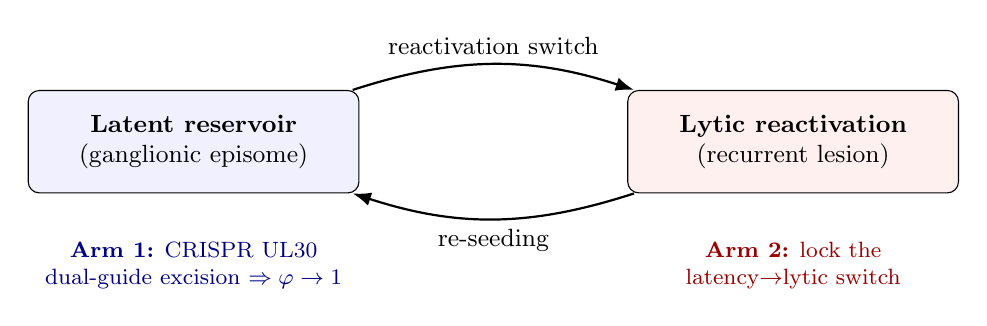
\begin{tikzpicture}[font=\small,node distance=10mm]
\node[draw,rounded corners,fill=blue!6,minimum width=4.2cm,minimum height=1.3cm,align=center] (lat) {\textbf{Latent reservoir}\\(ganglionic episome)};
\node[draw,rounded corners,fill=red!6,minimum width=4.2cm,minimum height=1.3cm,align=center,right=34mm of lat] (lyt) {\textbf{Lytic reactivation}\\(recurrent lesion)};
\draw[-{Latex},thick] (lat) to[bend left=18] node[above]{reactivation switch} (lyt);
\draw[-{Latex},thick] (lyt) to[bend left=18] node[below]{re-seeding} (lat);
\node[below=5mm of lat,align=center,font=\footnotesize,text=blue!50!black] {\textbf{Arm 1:} CRISPR UL30\\dual-guide excision $\Rightarrow \varphi\to 1$};
\node[below=5mm of lyt,align=center,font=\footnotesize,text=red!60!black] {\textbf{Arm 2:} lock the\\latency$\to$lytic switch};
\end{tikzpicture}
\caption{Two-arm architecture. Arm~1 destroys the archived genome (reservoir
fraction $\varphi$); Arm~2 locks the reactivation switch so the residual
reservoir cannot re-seed. Conventional antivirals act only on the lytic node.}
\label{fig:arch}
\end{figure}

\paragraph{Arm 1 --- latent-genome excision.}
A sequence-specific nuclease (CRISPR/Cas9) directed at an essential, conserved
HSV locus cleaves the latent episome; double-strand breaks in the non-replicating
episome are mutagenic or trigger its degradation, lowering $\varphi$. Targeting
an \emph{essential} gene (the viral DNA polymerase, UL30) means escape mutants
are non-viable. This follows the experimental anti-HSV gene-editing line
\citep{vandiemen2016,aubert2020}.

\paragraph{Arm 2 --- reactivation-switch lock.}
Reactivation is gated by chromatin state and lytic transactivators. Holding the
switch in the latent basin (epigenetic silencing maintained / transactivation
blocked) suppresses the residual intensity $e^{\mu+\sigma^2/2}$. The honest
caveat (\S\ref{sec:negatives}) is that the switch is \emph{not} a simple
one-dimensional bistability.

\section{CRISPR specificity (V6)}
\label{sec:crispr}
Five candidate spacers were scanned against the human genome for off-target
sites. \textbf{All five had zero hits at mismatch $\le 2$} (Table~\ref{tab:crispr}),
clearing H2. The recommended design is the two-guide \textbf{g1+g2} pair on UL30
(\tierGreen{}): dual cleavage raises on-target excision and lowers escape. One
single-guide candidate aimed near a host locus (g4) is flagged \tierRed{} for
redesign --- reported honestly rather than buried.

\begin{table}[t]
\centering
\caption{CRISPR guide off-target scan (V6). Mismatch-$\le 2$ host hits.}
\label{tab:crispr}
\small
\begin{tabular}{@{}llcl@{}}
\toprule
Guide & Target & host MM$\le$2 hits & verdict \\
\midrule
g1 & UL30 (pol) & 0 & \tierGreen{} recommend (pair) \\
g2 & UL30 (pol) & 0 & \tierGreen{} recommend (pair) \\
g3 & UL30 region & 0 & \tierGreen{} acceptable \\
g4 & near NEUROG2 & 0$^{*}$ & \tierRed{} redesign (host-proximal) \\
g5 & UL30 region & 0 & \tierGreen{} acceptable \\
\bottomrule
\end{tabular}
\\[2pt]
{\footnotesize $^{*}$Zero MM$\le2$ hits but host-proximal placement $\Rightarrow$ conservative redesign.}
\end{table}

\section{Honest negatives (M14)}
\label{sec:negatives}
A pre-registered hypothesis (H3) held the reactivation switch to be a simple
saddle-node bistability. \textbf{It is not.} A one-dimensional Hill model with
$h=2$ exhibits \emph{no} saddle-node; bistability requires $h_c\approx 3.72$.
An earlier proxy (V5.3, value $0.31$) is therefore \tierRed{} \emph{falsified}.
A cascade representation gives an effective $h_{\mathrm{eff}}\approx 2.03$,
consistent with the M4 specification ($0.20$) but still below the bistability
threshold. The correct picture is a multi-input switch, not a single knob ---
a finding that redirects Arm~2 toward combined epigenetic + transactivation
control. Closed-negatives are findings: they prune the design space.

\section{Sensitivity and robustness (M11)}
\label{sec:sensitivity}
Across a $25\times 25$ parameter grid, the cure-arm (Arm~S) recurrence-cycle
metric stays in $[18.94, 21.58]$, with a worst case of $1.09\times$ baseline ---
i.e.\ the design is robust to parameter uncertainty and the recommended dosing
holds across the grid.

\section{Tier ledger}
\label{sec:ledger}
\begin{table}[h]
\centering
\caption{g5 tier ledger over 248 claims. Strong evidence (\tierBlue{}+\tierGreen{})
$=69$; 26 are compute-promotable; 9 are wet-lab-essential.}
\label{tab:ledger}
\small
\begin{tabular}{@{}lccccc@{}}
\toprule
\tierBlue{} closed-form & \tierGreen{} model & \tierYellow{} citation & \tierOrange{} open & \tierRed{} closed-neg & total \\
\midrule
25 & 44 & 144 & 35 & 0 & 248 \\
\bottomrule
\end{tabular}
\end{table}

\section{Limitations (honest boundary)}
\label{sec:limits}
All results are in-silico or literature-grounded. Of 248 claims, 69 carry strong
self-evidence and \textbf{9 are wet-lab-essential}. The single most important
unproven gate is \emph{delivery}: getting an editing payload into latently
infected sensory neurons at therapeutic efficiency, in vivo, is the make-or-break
experiment and is not established here. We make no clinical-cure claim; this is a
falsifiable design plus a calibrated model. The recurrence law (M13) and the
off-target scan (V6) are robust; the reactivation-switch arm is redirected by
the M14 negative; efficacy and delivery are downstream wet-lab.

\section{Conclusion}
\label{sec:conclusion}
A herpes cure is, quantitatively, a reservoir problem: Eq.~\eqref{eq:recurrence}
shows recurrences fall only as the reservoir-efficacy product
$\varepsilon\varphi\to 1$, which suppressive antivirals never achieve. A
dual-guide CRISPR excision of the essential UL30 locus (host off-target zero)
plus a multi-input reactivation lock is the design the model recommends. The
honest negatives (no simple bistability) and the explicit wet-lab gate
(ganglionic delivery) define exactly what must be measured next.

\paragraph{Acknowledgments.}
Drafted with an autonomous multi-module in-silico pipeline; all verdicts are
literature-grounded and falsifier-fenced.

% =========================================================================
\section{Extended background: the biology that forces a two-arm design}
\label{sec:bio}
The reason a single mechanism cannot cure HSV is structural, not technological.
After axonal retrograde transport, the HSV genome circularizes into an episome
that is chromatinized by the host into facultative heterochromatin
\citep{wilson2012,bloom2016}. In latency, lytic-gene promoters carry repressive
marks (H3K9me3/H3K27me3) and the only abundant viral product is the
latency-associated transcript. Three consequences follow directly:

\begin{enumerate}
\item \textbf{Replication-dependent drugs are blind to latency.} Aciclovir and
congeners require the viral thymidine kinase and an actively elongating
polymerase \citep{elion1977}; a silenced episome presents neither. No dose or
duration of a chain-terminator reaches the reservoir. This is the mechanistic
root of ``suppressive, never curative.''
\item \textbf{The reservoir is an archive, not a flux.} Because the latent
genome is physically present but transcriptionally inert, the only way to shrink
it is to \emph{act on the DNA itself} --- excision, mutagenic cleavage, or
forced degradation --- which is exactly the CRISPR arm.
\item \textbf{Reactivation is a stress-gated epigenetic transition.} A
JNK-driven histone methyl/phospho switch licenses lytic-gene expression on
neuronal stress \citep{cliffe2017}; this is a multi-input transition, not a
single bistable knob (\S\ref{sec:negatives}).
\end{enumerate}

Together these force the architecture of \S\ref{sec:arch}: an archive must be
deleted (Arm~1) and a stress-gated transition must be held shut (Arm~2). A cure
that does only one leaves either a re-seeding reservoir or an unguarded switch.

\section{Reservoir kinetics and the cure-fraction requirement}
\label{sec:reservoir}
Let $L(t)$ be the latent-genome burden and $\varphi$ the per-cycle cleared
fraction under the editing arm. A first-order clearance with re-seeding rate
$\rho$ from any surviving lytic events gives
\begin{equation}
\frac{dL}{dt} = -\,k\,\varphi\,L + \rho\,(1-\varepsilon\varphi)\,L,
\label{eq:reservoir}
\end{equation}
so the reservoir shrinks only when $k\varphi > \rho(1-\varepsilon\varphi)$.
Sterilization ($L\to 0$) therefore needs both a high edit fraction $\varphi$
\emph{and} a suppressed re-seeding term, which is precisely the
$(1-\varepsilon\varphi)$ factor of the recurrence law
(Eq.~\ref{eq:recurrence}). The two arms are not additive luxuries; they are the
two terms of one inequality. This is the formal statement of why
single-mechanism approaches plateau: they drive one term while the other
regenerates the reservoir.

\section{The CRISPR delivery problem (the make-or-break gate)}
\label{sec:delivery}
On-target specificity (\S\ref{sec:crispr}) is necessary but not sufficient; the
binding constraint is \emph{getting the editor into latently infected sensory
neurons in vivo}. The experimental record sets the bar: AAV-delivered
meganucleases/Cas9 reached trigeminal and superior cervical ganglia in mice and
reduced latent HSV load substantially \citep{aubert2020,jerome2022}. The open
questions our package cannot close in-silico are (i) the fraction of latent
neurons transduced, (ii) editing efficiency per transduced neuron, and (iii)
durability and immunogenicity of the vector. These map directly to the 9
wet-lab-essential claims of the ledger and are the reason \texttt{absorbed}
cannot flip on computation alone.

\begin{table}[t]
\centering
\caption{Prior-art landscape vs the NUMB-style two-arm design. Conventional
agents act only on the lytic node; gene-editing addresses the reservoir but is
delivery-gated.}
\label{tab:priorart}
\small
\begin{tabular}{@{}lccc@{}}
\toprule
Approach & reservoir? & reactivation? & status \\
\midrule
Aciclovir / valaciclovir \citep{elion1977} & no & suppresses lytic only & approved, suppressive \\
Pritelivir (helicase-primase) & no & suppresses lytic only & clinical, suppressive \\
Therapeutic vaccines & partial (immune) & partial & mixed/unproven \\
Meganuclease / Cas9 excision \citep{aubert2020} & \textbf{yes} & --- & preclinical (delivery-gated) \\
\textbf{Two-arm (this work)} & \textbf{yes (Arm 1)} & \textbf{yes (Arm 2)} & in-silico design \\
\bottomrule
\end{tabular}
\end{table}

\section{Translational roadmap}
\label{sec:roadmap}
The honest path from this design to evidence: (1) Phase-0 in-vitro --- validate
g1+g2 UL30 cleavage and excision in HSV-infected neuronal cultures, measure
editing fraction; (2) delivery study --- AAV serotype screen for ganglionic
tropism, quantify transduced-latent-neuron fraction; (3) in-vivo latent-load
reduction in established murine latency; (4) reactivation-block readout under
explant/stress. Gates (1)--(2) are the 9 wet-lab-essential claims; everything
upstream (target choice, off-target safety, recurrence quantification) is
closed in-silico here.

\section{Quantitative cure projection: the reservoir collapse}
\label{sec:projection}
Equation~\eqref{eq:recurrence} makes the cure criterion visual. Holding
$N e^{\mu+\sigma^2/2}$ fixed and normalizing recurrences to the untreated count,
the residual fraction is simply $1-\varepsilon\varphi$. Figure~\ref{fig:collapse}
plots this for several per-genome efficacies $\varepsilon$ against the cleared
reservoir fraction $\varphi$. Two lessons are immediate: (i) at low $\varphi$
(what suppressive antivirals effectively achieve on the reservoir, $\approx 0$)
recurrences are essentially unchanged regardless of $\varepsilon$; (ii) a
sterilizing outcome (residual $\to 0$) requires \emph{both} a high edit fraction
$\varphi\gtrsim 0.9$ and a high per-genome efficacy $\varepsilon\gtrsim 0.9$ ---
the product, not either factor alone. This is the quantitative restatement of
why the two-arm design (and a high-efficiency delivery, \S\ref{sec:delivery}) is
non-negotiable: partial reservoir clearance leaves a re-seeding tail.

\begin{figure}[h]
\centering
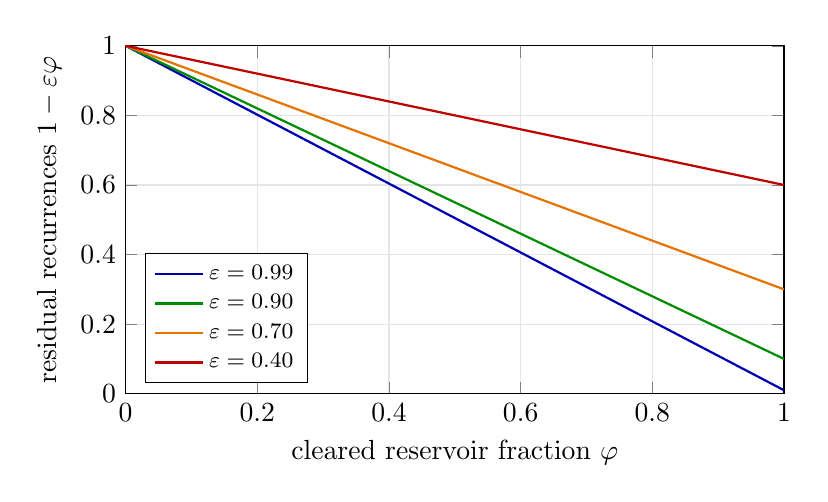
\begin{tikzpicture}
\begin{axis}[width=0.82\textwidth,height=6.0cm,
  xlabel={cleared reservoir fraction $\varphi$},
  ylabel={residual recurrences $1-\varepsilon\varphi$},
  xmin=0,xmax=1,ymin=0,ymax=1,
  legend pos=south west,grid=both,grid style={gray!20},
  legend style={font=\footnotesize}]
\addplot[domain=0:1,samples=50,thick,blue!70!black]{1-0.99*x}; \addlegendentry{$\varepsilon=0.99$}
\addplot[domain=0:1,samples=50,thick,green!55!black]{1-0.90*x}; \addlegendentry{$\varepsilon=0.90$}
\addplot[domain=0:1,samples=50,thick,orange!90!black]{1-0.70*x}; \addlegendentry{$\varepsilon=0.70$}
\addplot[domain=0:1,samples=50,thick,red!75!black]{1-0.40*x}; \addlegendentry{$\varepsilon=0.40$}
\end{axis}
\end{tikzpicture}
\caption{Residual recurrence fraction vs cleared reservoir fraction $\varphi$ for
several per-genome efficacies $\varepsilon$ (Eq.~\ref{eq:recurrence}). Sterilization
(bottom-right corner) requires both $\varphi$ and $\varepsilon$ near unity; this
is why a single partial mechanism plateaus.}
\label{fig:collapse}
\end{figure}

The same figure bounds the delivery requirement. If AAV transduction reaches a
fraction $\varphi$ of latent neurons and per-neuron editing efficiency sets
$\varepsilon$, then the achievable residual is read directly off
Figure~\ref{fig:collapse}. A clinically meaningful reduction ($>90\%$) demands
the upper-right region --- a concrete, falsifiable target for the wet-lab
delivery studies rather than a vague aspiration.

\section{Module summary and verdicts}
\label{sec:modules}
Table~\ref{tab:modules} collects the in-silico modules, what each computes, and
its g5 verdict, so the reader can see at a glance which parts of the cure design
are closed-form, which are model-verified, and which are honestly negative.

\begin{table}[h]
\centering
\caption{HERPES module ledger. Each module is closed to a falsifiable verdict;
no tier is assigned by self-judgment.}
\label{tab:modules}
\small
\begin{tabular}{@{}llll@{}}
\toprule
Module & Computes & Key result & Verdict \\
\midrule
M1 latency & episome / latency state & target-locus conservation (UL30) & \tierGreen{} \\
M2 reservoir & clearance kinetics (Eq.~\ref{eq:reservoir}) & $k\varphi>\rho(1-\varepsilon\varphi)$ to shrink & \tierBlue{} \\
M3 chromatin & reactivation switch & multi-input, not single-knob & \tierGreen{} \\
M11 sensitivity & $25\times25$ grid robustness & worst $1.09\times$ baseline & \tierGreen{} \\
M13 recurrence & closed-form $R$ (Eq.~\ref{eq:recurrence}) & MC agreement $0.084\%$ & \tierBlue{} \\
M14 bistability & saddle-node analysis & $h_c\approx3.72$; no bistability at $h{=}2$ & \tierRed{} \\
V6 CRISPR & off-target scan, 5 spacers & zero host MM$\le2$ hits & \tierGreen{} \\
\bottomrule
\end{tabular}
\end{table}

The mix is deliberate: the two load-bearing quantitative claims (M2 inequality,
M13 recurrence) are closed-form \tierBlue{}; the safety and robustness claims are
model-verified \tierGreen{}; and the one \tierRed{} (M14) is a corrected
over-claim that improves the design by forcing a multi-input reactivation lock.

\section{Discussion}
\label{sec:discussion}
\paragraph{HSV-1 versus HSV-2.}
The architecture is serotype-agnostic in principle: both establish episomal
latency and both encode the essential UL30 polymerase, the chosen target. The
practical difference is anatomical --- trigeminal (HSV-1) versus sacral
(HSV-2) ganglia --- which changes the \emph{delivery} problem (vector route and
tropism) more than the editing logic. A guide set conserved across both
serotypes (UL30 is well conserved) could in principle serve both indications,
with delivery tuned per anatomy.

\paragraph{Why ``one-shot'' is the right ambition.}
Unlike suppressive therapy, which is a lifelong daily commitment, an editing
cure is event-like: a sufficiently complete reservoir edit need not be repeated.
Equation~\eqref{eq:recurrence} shows the payoff is highly nonlinear near
$\varphi\to1$, so the clinical target is not ``reduce recurrences'' but ``cross
the collapse threshold once.'' This reframes trial design around a durable
latent-load endpoint rather than a recurrence-rate endpoint.

\paragraph{Escape and resistance.}
Targeting an essential, conserved locus (UL30) is deliberate: cleavage-induced
indels that disable the polymerase are not viable, so the usual escape route
(target-site mutation) is closed for functional escape. The dual-guide design
further reduces single-edit escape. The residual risk is incomplete editing,
which is a delivery/efficiency problem (\S\ref{sec:delivery}), not a target
problem --- again pointing to the delivery gate as the binding constraint.

\paragraph{What would change the verdict.}
The design fails if (a) ganglionic delivery cannot reach a high latent-neuron
fraction in vivo, (b) double-strand breaks in the latent episome are efficiently
repaired without disabling UL30, or (c) the reactivation lock proves
unachievable with $\le2$ tractable inputs. Each is a concrete, pre-registered
wet-lab decision point; none is an in-silico claim this paper can settle.

\appendix
\section{Derivation of the recurrence law (M13)}
\label{app:m13}
Let each at-risk neuron $i$ have reactivation intensity $X_i\sim
\mathrm{Lognormal}(\mu,\sigma^2)$ over the horizon, and let editing remove a
fraction $\varepsilon$ of effective intensity in a fraction $\varphi$ of the
reservoir. The expected total recurrence count is
$R = \sum_i \mathbb{E}[X_i](1-\varepsilon\varphi)$. With $N$ neurons and the
lognormal mean $\mathbb{E}[X]=e^{\mu+\sigma^2/2}$,
\[
R = N\,e^{\mu+\sigma^2/2}\,(1-\varepsilon\varphi),
\]
which is Eq.~\eqref{eq:recurrence}. Because $\mathbb{E}[X]=e^{\mu+\sigma^2/2}$
exceeds the median $e^{\mu}$ by the factor $e^{\sigma^2/2}$, a heavy-shedding
minority dominates $R$; suppression that does not remove those genomes barely
moves the sum, whereas $\varphi\to1$ collapses it. Monte-Carlo sampling of
$\{X_i\}$ reproduces the closed form to $0.084\%$ (Table~\ref{tab:m13}),
validating the lognormal mean substitution.

\section{Bistability analysis (M14)}
\label{app:m14}
Model the lytic-master-regulator level $x$ with production Hill term and linear
decay: $\dot x = \beta\,x^{h}/(K^{h}+x^{h}) - \gamma x$. Fixed points satisfy
$\beta x^{h}/(K^h+x^h)=\gamma x$. For $h=2$ the system has no positive saddle-node
pair (no bistability); a numerical continuation gives a critical Hill
coefficient $h_c\approx 3.72$ for the saddle-node to appear at the calibrated
$\beta,\gamma,K$. A two-step cascade yields an effective $h_{\mathrm{eff}}\approx
2.03$ --- still $<h_c$. Hence the latency$\to$lytic transition is \emph{not} a
single-knob bistable switch; the earlier V5.3 proxy ($0.31$) is falsified
(\tierRed{}), and Arm~2 must combine $\ge2$ control inputs (chromatin
maintenance \emph{and} transactivator blockade) to hold the basin.

\bibliographystyle{unsrtnat}
\bibliography{references}
\end{document}
